\documentclass[openany]{book}
\input{notes_light}
\usepackage{mathtools}
\settitle{Computability Notes}
\begin{document}

\title{\Large{\underemphasise{Recursion, Computability and Algorithms Notes}} \\ \vspace{5pt}
\large{An exploration of the beautiful topic of recursive functions, computability, algorithms and The Incompleteness Theorems}}
\author{Eklavya Raman}
\date{\today}
\maketitle
\tableofcontents
\listoftheorems[
    show=mytheorem,
    title={List of Theorems}]
\part{Theory of Recursive Functions and Effective Computability}
\chapter{Recursive Functions}


\section{Algorithms}
\subsection{What is an algorithm?}
Algorithms are sets of instructions of a given finite size. We need computing agents, storage facilities for executing the algorithms and managing, storing the inputs and instructions. The instructions are carried out in a stepwise and deterministic way by the computing ag ent which is usually a human.
\begin{mydefinition}{Deterministic Process}
    A deterministic process is one which does not rely on random methods, i.e. dice. In other words it follows a set of known and predictable steps. 
\end{mydefinition}
\begin{mydefinition}{P and LP Symbolism}
Here we define both in terms of sets of symbolic expressions and their meanings, in a sense. 
\begin{itemize}
    \item P symbolisms are the specifics sets of symbolic expressions accepted as instructions, inputs, or outputs. 
    \item How the above instructions and inputs determine how we can compute and identify outputs is know as LP Symbolism. 
\end{itemize}
\end{mydefinition}
\subsection{What are the boundations of an Algorithm?}
Lets begin by simple statements - 
\begin{enumerate}
    \item Theoretically, there does not need to be a fixed finite bound on the size of inputs, that is, we can have an arbitrarily large set of inputs or inputs that are arbitrarily large. 
    \item Theoretically, there does not need to be a fixed finite bound on the size of the set of instructions, that is, we can have an arbitrarily large number of instructions. 
    \item Therefore it follows that, theoretically, there does not need to be a fixed finite bound on the size of memory or storage available. 
\end{enumerate}
However, in a practical scenario, we encounter two types of functions - 
\begin{enumerate}
    \item \textbf{Functions computable by finite-state machine} - These can be computed using a finite state machine (a machine with finite memory capacity), no matter the size of the inputs. \\
    For example - $\lambda x[2x]$ as $x$ increases.
    \item The converse of the above. \\
    For example - $\lambda x[x^2]$ as $x$ increases. 
\end{enumerate}
We must also note the following - 
\begin{itemize}
    \item There is to be a fixed finite bound on the capacity of the ability of the computing agent (L). 
\end{itemize}
\begin{mynote}
\textbf{Limiting the Computing Agent (L)} \\
With a sufficiently flexible P-symbolism, meaning that we can modify the P-symbolism such that excessive computing capacities of L are converted to demands on the memory capacity, we can limit L. The ways are enlisted below - 
\begin{enumerate}
    \item Limit L to simple clerical operations. 
    \item A temporary memory of fixed size which preserves the 'place' we have reached within the set of instructions or inputs. 
    \item A set of rules to determine the next state of the temporary memory and the next clerical operation to be performed. 
\end{enumerate}
This becomes clearer when we consider \underemphasise{Turing Machines} later in the notes. 
\end{mynote}
Lastly, we require that computation ends after some finite number of steps. 
\section{Primitive Recursive Functions}
\subsection{What are recursive functions?}
\begin{mydefinition}{Recursive Functions}
Functions obtainable by a recursive definition, that is, values of the functions for given arguments are directly related to values of the same functions for simpler arguments (most usually a set of base constant values). 
Recursive functions can often be made to serve as algorithms. 
\end{mydefinition}
The finest and most beautiful example of a recursive function is the \textbf{\textit{Fibonacci Sequence}}. \\
\begin{example}
$f: \N \xrightarrow{} \N$ given by - 
    \begin{align*}
        &f(0) = 1 \\
        &f(1) = 1 \\
        &f(x+2) = f(x+1) + f(x)
    \end{align*}
The algebraic definition of the fibonacci sequence is - 
$$f(x) = \frac{\sqrt{5}}{5}\left({\frac{1+\sqrt{5}}{2}}\right)^{x+1} - \frac{\sqrt{5}}{5}\left({\frac{1-\sqrt{5}}{2}}\right)^{x+1}$$
\end{example}
\begin{mydefinition}{Class of Primitive Recursive Functions}
Denoting by $\C$, the class includes - 
\begin{enumerate}
    \item All constant functions.
    \item The successor function.
    \item All identity functions. 
    \item If f is a function of k variables in $\C$ and $g_1, g_2, ..., g_k$ are each functions of m variables in $\C$, then the function - 
    $$\lambda x_{1}, x_{2}...x_{m}[f(g_{1}(x_{1}, ..., x_{m}), ..., g_{k}(x_1, ..., x_{m}))]$$ is also in $\C$.
    \item If h is a function of k+1 variables in $\C$ and g is a function of k-1 variables in $\C$, then the unique function f of k variables satisfying - 
    \begin{align*}
        &f(0, x_2, ..., x_k) = g(x_2, ..., x_k) \\ 
        &f(y+1, x_2, ..., x_k) = h(y, f(y, x_2, ..., x_k), x_2, ..., x_k)
    \end{align*}
    is also in $\C$
\end{enumerate}
\end{mydefinition}
\begin{mynote}
    The above definition leads to the fact that - \\
    For any f, f is primitive recursive $\iff$ there is a finite sequence of functions $f_1, f_2, ... f_n$ such that $f_n = f$ and for each $j\leq n$, $f_j$ is in $\C$ pr is directly obtainable from some of the $f_i$, $i \leq j$ using 4. or 5. 
    Almost all algorithmic functions in ordinary mathematics can be shown to be primitive recursive. 
\end{mynote}
\begin{mydefinition}{Derivation}
    If a sequence as mentioned above is described with a specification of how each function in the sequence is obtained, we say that we have a derivation for f as a primitive recursive function. 
\end{mydefinition}
\begin{mynote}
    For more on the usefulness of primitive recursiveness, Peter [1951, pp. 1-67]
\end{mynote}
Even if primitive recursive functions are quite accurate, they are not completely generalized and do not work for all functions computable by algorithm. Example is the \textit{Ackermann Generalized Exponential} function. Hence these are not accurate formal counterpart to the notion of algorithmic function. \\ 
We can also provide functions that we can prove have an algorithmic derivation but we do not know yet how to find the derivation. \\
\begin{example}
    \textbf{Goldbach's Conjecture} - The conjecture states that every even number greater than 2 is the sum of 2 primes. We define a function h by - 
    $$h(x) = \begin{dcases}
        1 & \text{if conjecture true;} \\
        0 & \text{otherwise} \\
    \end{dcases}$$
    It is enough to see that h is a constant function to conclude that it is indeed primitive recursive. However, we do not know how to identify the correct derivation. 
\end{example}
\subsection{Diagonalization}
This is similar to the Diagonilazation argument by Cantor. It is a method applied to formal classes of algorithmic functions wchi produces a function outside of the formal class. The diagonalization arguments suggests that we can not have a P-Symbolism and LP-Symbolism strong enough to represent all algorithmic functions. 
\begin{mynote}
    Diagonalization presents an interesting possible relation to Godel's Incompleteness theorems.
\end{mynote}
\subsubsection{Formal Characterization}
\begin{mynote}
    We can avoid Diagonilaztion by allowing sets of instructions for partial functions as well as for total functions. Basically, we allow procedures which don not always terminate and yield an output, i.e. partial functions. 
\end{mynote}
The approach of introducing a class of partial functions was taken first by Kleene, Church, and Turing. The common features of the characterizations of these different researchers were - 
\begin{enumerate}
    \item Formal counterparts to the notion of an Algorithm through P-symbolisms. 
    \item Formal counterparts for the notion of a partial function computable by algorithm.
\end{enumerate}
\subsection{Fun Interlude}
\begin{mycodeblock}
\begin{lstlisting}[language=Python, caption={Brute Force Algorithm to verify Goldbach's Conjecture}]
import itertools
def is_prime(n):
    if n == 1:
        return False
    elif n == 2:
        return True
    elif n == 3:
        return True
    elif n == 4:
        return False
    else:
        for i in range(2, int(n//2)):
            if n % i == 0:
                return False
    return True

def is_even_geq_2(n):
    if n <= 2:
        return False
    elif n%2!=0:
        return False
    else:
        return True

def verify(n):
    primes = []
    for i in range(2, n + 1):
        if is_prime(i):
            primes.append(i)
    combinations = list(itertools.product(primes, repeat=2))
    for i in combinations:
        a = 0
        for j in i:
            a += j
        if a == n:
            return True
        else:
            a = 0
    return False

def soln(n):
    for i in range(1, n + 1):
        if is_even_geq_2(i):
            if verify(i):
                pass
            else:
                return False
    return True
\end{lstlisting}
\end{mycodeblock}
\begin{figure}[h]
\centering
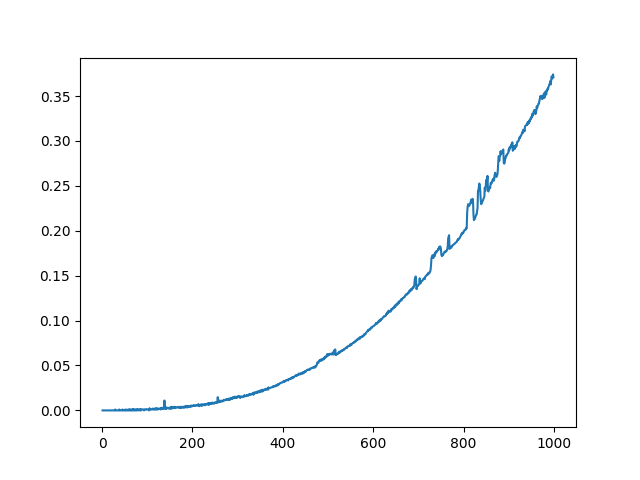
\includegraphics[width=\textwidth]{images/Goldbach_Conjecture_1.png}
\caption{Runtime in secs for the first 1000 integers}
\end{figure}
We can notice some interesting peaks and valleys in an otherwise smooth graph. To be looked at later.
\subsection{Turing Characterization}
We consider first a physical picture of the Turing Characterization for the purpose of illustration. \\
Let us say we have a machine that can perform 4 operations - A, B, C, D. It performs 1 operation per unit time. The device can take on one of a fixed finite set of possible mechanical configurations called the \textbf{Internal State}. The device must follow a set of deterministic rules. \\
Let there be 2 possible, that is binary conditions for the cell being examined by the machine. Then the set of rules determining the behavior of the device may be expressed as \textbf{\textit{quadruples}} that include the internal state, the condition of the cell, an operation and a further internal state. To ensure consistency, we require that for each internal state and cell condition, there is exactly one quadruple.
\begin{mydefinition}{Turing Machine}
    A Turing Machine is a device that can perform a set of operations on a set of inputs, and can be described by a set of quadruples as described above, provided that the consistency condition is satisfied, and the set of quadruples is constructed using a finite number of internal states. \\ 
    A more rigorous definition is given as follows - \\
    Let $T= {0, 1}$ and $S = {0, 1, 2, 3}$. Then a Turing Machine can be defined as a mapping from a finite subset of $\N \times T$ into $S \times \N$
\end{mydefinition}
\begin{mynote}
    The Turing Machine is a physical model of computation, and is not a formal model. It is a model of a computing agent that can perform operations on inputs and outputs in a deterministic manner.
\end{mynote}

\begin{mydefinition}{Turing Computable Function}
    A function is Turing computable if there exists a Turing Machine that can compute the function.
\end{mydefinition}
\begin{example}
We verify that the function $\lambda x[2x]$ is yielded by the following Turing Machine -  
\begin{align}
    &q_{0}1Bq_1 \\
    &q_{1}BRq_2 \\
    &q_{2}1Bq_3 \\
    &q_{3}BRq_4 \\
    &q_{4}1Rq_4 \\
    &q_{4}BRq_5 \\
    &q_{5}1Rq_5 \\
    &q_{5}B1q_6 \\
    &q_{6}1Rq_6 \\
    &q_{6}B1q_7 \\
    &q_{7}1Lq_7 \\
    &q_{7}BLq_8 \\
    &q_{8}1Lq_1 \\
    &q_{1}1Lq_1
\end{align}
The machine takes a tape with x+1 consecutive 1s and outputs 2x+1 1s. $q_0$ is the leftmost cell containing 1. Let the input string be - \\
$$...B111B...$$
Following the above quadruples, we can see that the machine will output -
$$...B11111B...$$
\end{example}
Turing Machines, like other characterizations, give a class of algorithmic partial functions. The class may seem to be limited, but it provides a meaningful P-symbolism and LP specifications. 
\subsection{Kleene Characterization}
Kleene's characterization is very much similar to the kind we used in example 1.2.1.1 to describe the Fibonacci sequence. The Kleene characterization is a formalization of the idea of a recursive function. It is based on the idea of a recursive definition, where the value of a function for a given argument is defined in terms of the values of the same function for simpler arguments. The P symbolism is the same as the one used to describe functions, equations, and variables in general mathematics, \underemphasise{except that for describing a term such as $x+2$, we must write $x + 1 + 1$}. 
\begin{mynote}
    Every primitive recursive function can be expressed in Kleene's notation or the P-symbolism of the Kleene Characterization. As such we can find a \emphasise{derivation} for every primitive recursive function in Kleene's notation.
\end{mynote}
\subsubsection{Limitations of Kleene's Characterization}
Kleene's Characterization does not guarantee that the computation is uniquely determined by the input or that one input may yield multiple outputs. It also does not guarantee that an output will be generated for every input. \\
To avoid such limitations, we do the following - \\
Given any P, we generate a list of all equations deducible from P. Then for the given P and any input, we define the \emphasise{principal output} as the first output that can be deduced from the list of equations. We only allow one principal output for each input.  \\
\begin{mynote}
    Note that the above characterization also forms a class of algorithmic partial functions, similar to the Turing Characterization.  
\end{mynote}
\section{The Basic Result}
The following is a fundamental result, which will be used throughout the rest of the notes. It is a result that shows the equivalence of the different characterizations of algorithmic functions.
\subsection{Partial Recursive Functions}
\begin{mytheorem}[The Basic Result - 1]
    \underemphasise{The Basic Result - 1} \\
    The proposed characterizations of algorithmic functions by Turing, Kleene, and others are equivalent in the sense that they yield the same class of algorithmic partial functions. \\
\end{mytheorem}
\begin{mydefinition}{Partial Recursive Functions}
    A function is said to be a partial recursive function if it is computable by a Turing Machine, or if it is computable by a Kleene Characterization, or if it is computable by any other characterization of algorithmic functions. \\
    That is, it is the class of partial functions (and hence total functions) generated by the formal characterizations as mentioned above. 
\end{mydefinition}
\begin{mytheorem}[The Basic Result - 2]
    \underemphasise{The Basic Result - 2} \\
    A wide variety of partial functions have been shown to be partial recursive functions. \emphasise{Theorem 1.3.1.1} and this provides evidence that the class of partial recursive functions is inclusive of a large number of functions computable by algorithm. 
\end{mytheorem}
\begin{mytheorem}[The Basic Result - 3]
    \underemphasise{The Basic Result - 3} \\
    Given any set of insctructions P from one characterizations, we can find a set of instructions P' from another characterization for the same partial function. 
\end{mytheorem}
\subsection{Church's Thesis}
\begin{mytheorem}[Church's Thesis]
    \underemphasise{Church's Thesis} \\
    We accept, on empirical  grounds, that the characterizations mentioned above are satisfactory formalizations of the notion of algorithms and algorithmic functions.
\end{mytheorem}
\begin{mynote}
    This book relies on the Church's Thesis, and its assumption, to provide informal but rigorous proofs of the results presented in the book. \\
    The Church's Thesis is not a theorem, but an assumption that is widely accepted in the field of computability. It is based on the empirical evidence that the characterizations mentioned above are sufficient to describe all algorithmic functions.\\
    It should also be noted that there are ways to formally construct the same proofs that have been developed informally. The formal proofs are not presented in this book, but the informal proofs are rigorous and provide a good understanding of the results. 
\end{mynote}
\section{Godel Numbers, Universality, s-m-n Theorem}
\subsection{Godel Numbers}
Assume we can list all the sets of instructions P from one characterization. Such a procedure associates an integer x with the $(x+1)^{th}$ set of instructions in the list of all sets of instructions. 
\begin{mydefinition}{Godel Number}
    A Godel Number is an integer that is associated with a set of instructions P from one characterization. It is used to identify the set of instructions in the list of all sets of instructions. It is also sometimes referred to as the \emphasise{index} of the set of instructions. \\ 
    Let $P_x$ be the set of instructions associated with the Godel Number $x$. Then, the partial function computable by the set of instructions $P_x$ is denoted by $\varphi_x^k$. Thus, $x$ is also the \emphasise{index} or \emphasise{Godel Number} for the partial function associated with $P_x$.  
\end{mydefinition}
\begin{mytheorem}[Countability of Recursive Functions]
    There are exactly \emphasise{$\aleph_0$} Godel Numbers (since there are countably many sets of instructions). Therefore, there are countably many partial recursive functions and countably many recursive functions. 
\end{mytheorem}
\begin{proof}
    The proof is based on the fact that there are countably many sets of instructions, and hence countably many Godel Numbers. Since each Godel Number is associated with a set of instructions, and each set of instructions can be used to compute a partial recursive function, it follows that there are at most countably many partial recursive functions. \\
    Since all constant functions are recursive, there are at least countably many recursive functions. Therefore, there are exactly countably many recursive functions.
\end{proof}
\begin{mytheorem}[Existence of Non-Recursive Functions]
    There exist functions that are not recursive.
\end{mytheorem}
\begin{proof}
    We succeeded in showing there are exactly $\aleph_0$ recursive functions. By Cantor's Theorem, there exist \emphasise{$2^{\aleph_0}=\aleph_1$} many functions. Hence, by PHP, there must exist function(s) that are not recursive. 
\end{proof}
\begin{mytheorem}[Countability of Indices]
    Each partial recursive function has $\aleph_0$ indices or Godel Numbers. 
\end{mytheorem}
\begin{proof}
    Let the partial recursive function be $\varphi_{x_0}$. Let $P_{x_0}$ be the set of instructions associated with $\varphi_{x_0}$. Let m-1 denote the highest subscript integer of any internal state in $P_{x_0}$. Then we can modify $P_{x_0}$ by adding redundant quadruples - $q_{m}11q_m$, $q_{m+1}11q_{m+1}$, ... $q_{m+k}11q_{m+k}$ where $k$ is a positive integer. Depending on $k$, we get the unique set of instructions $P^{k}_{x_0}$. Since $k$ is a positive integer, we can have countably many sets of instructions for $\varphi_{x_0}$.
\end{proof}
\subsection{Universality}
\begin{mytheorem}[Enumeration Theorem]
    \underemphasise{Enumeration Theorem} \\
    There exists a partial recursive function $\Psi$ such that for every partial recursive function $\varphi_x$ and any $y$, $\Psi(x, y) = \varphi_x(y)$.
\end{mytheorem}
\begin{proof}
We define a function $\Psi$ algorithmically as follows - \\
Given $<x, y>$, find $P_x$ (This is itself algorithmic), then apply $P_x$ to $y$. If and when $\varphi_x(y)$ terminates, take the output as the output of $\Psi(x, y)$. If it does not terminate, then $\Psi(x, y)$ does not terminate. \\
Therefore, $\Psi$ can be defined as - 
$$\Psi(x, y) = 
\begin{dcases}
    \varphi_x(y) & \text{if } \varphi_x(y) \text{ converges} \\
    \text{divergent} & \text{otherwise}
\end{dcases}$$
By Church's Thesis, since $\Psi$ can be computed algorithmically, $\Psi$ is a partial recursive function. Hence, we can say that $\Psi = \varphi^{(2)}_{x_0}$ for some $x_0$, that is a partial recursive function of 2 variables with Godel Number $x_0$.
\end{proof}
The given proof can be generalized to show that there exists a partial recursive function $\Psi$ such that for every partial recursive function $\varphi^{(n)}_x$ and $y_1, y_2, ..., y_n$ - $$\Psi(x, y_1, y_2, ..., y_n) = \varphi_x(y_1, y_2, ..., y_n)$$ 
where $n$ is a positive integer. The function $\Psi$ is called a \underemphasise{universal partial function}.  
\begin{mynote}
An alternate way to denote the function is - \\
$$\Psi(x, y_1, y_2, ..., y_n) = \varphi^{(n+1)}_{x_1}$$ for some $x_1$. \\
The universal partial function essentially takes as input the Godel Number of a partial recursive function and the inputs to that function, and outputs the result of the function. In other words, it simulates the computation of any partial recursive function given its Godel Number and inputs.
\end{mynote}
\subsection{s-m-n Theorem}
\begin{mytheorem}[s-m-n Theorem]
\underemphasise{s-m-n Theorem} \\
For every $m, n \geq 1$, there exists a recursive function $s_n^m$ of $m+1$ variables such that for all  $x, y_1, y_2, ..., y_m$ -
$$\lambda z_{1}z_{2}...z_{n}[\varphi_{x}^{(m+n)}(y_1, y_2, ..., y_m, z_1, z_2, ..., z_n)] = \varphi^{(n)}_{s^{m}_{n}(x, y_1, y_2, ..., y_m)}$$
\end{mytheorem}
\begin{proof}
    Consider the family of all partial functions of n variables which are expressible as -  $$\lambda z_{1}z_{2}...z_{n}[\varphi_{x}^{(m+n)}(y_1, y_2, ..., y_m, z_1, z_2, ..., z_n)]$$ for some $x$ and $y_1, y_2, ..., y_m$. \\
    Note that this is a new formal characterization offor a class of partial recursive functions of $n$ variables. By \underemphasise{The Basic Result - 3}, there exists a effective procedure for going from sets of instructions in this new characterization to sets of instructions in our standard characterization. Therefore, there must be a recursive function $f$ of $n$ variables such that - 
    $$\lambda z_1, z_2... z_n[\varphi_{x}^{(m+n)}(y_1, y_2, ..., y_m, z_1, z_2, ..., z_n)] = \varphi^{(n)}_{f(x, y_1, y_2, ..., y_m)}$$
    This function $f$ is the function $s_n^m$. Here, we have generalized the proof given within the book.
\end{proof}
\begin{mynote}
In essence, the s-m-n theorem states that for every partial recursive function of $m+n$ variables, there exists a partial recursive function of $n$ variables that can be obtained by fixing the first $m$ variables. It is achieved by constructing a new characterization of partial recursive functions and then using the Basic Result to show the existence of a new set of instructions within the standard characterization that can compute the same function.\\ 
This new set of instructions is generated by computing the \underemphasise{s-n-m function} which takes as input the Godel Number of the original function and the fixed values of the first $m$ variables and outputs the Godel Number for the partial recursive function which computes the function for all values of $z_1, z_2, ..., z_n$ with fixed values of $x$ and $y_1, y_2, ..., y_m$. \\
\underemphasise{The s-m-n function is itself patial recursive.} 
\end{mynote}
\begin{mytheorem}[Composite of Partial Recursive Functions are Partial Recursive]
    There is a recursive function $g$ of 2 variables such that for all $x, y$ - 
    $$\varphi_{g(x, y)} = \varphi_x \circ \varphi_y = \lambda z[\varphi_x(\varphi_y(z))]$$
\end{mytheorem}
\begin{proof}
By \underemphasise{Church's Thesis}, for any given $x, y$, $f = \varphi_x \circ \varphi_y$ is a partial recursive function. This implies that there exists a Godel Number $g(x, y)$ such that $\varphi_{g(x, y)} = f$. \\
Define - 
$$\theta(x, y, z) = \varphi_{x_0}(x, \varphi_{x_0}(y, z)) = \varphi_x(\varphi_y(z))$$
where $x_0$ is the Godel Number of the universal partial function $\Psi$. Then, $\theta$ is a partial recursive function of 3 variables and therefore has a godel number, say $x_1$ \\
Then, by the \underemphasise{s-m-n Theorem}, we have -
$$\varphi_x\varphi_y=\lambda z[\varphi_{x_1}(x, y, z)] = \varphi_{s^2_1(x_1, x, y)}$$
where $s^2_1$ is the s-m-n function for $m=2$ and $n=1$. \\
$\lambda xy[s^2_1(x_1, x, y)]$ gives us $g(x, y)$. 
\end{proof}
\begin{mynote}
The main idea in the proof is to use the s-n-m theorem to construct a new partial recursive function that computes the composition of two partial recursive functions with previously defined Godel Numbers. First, we construct a function of three variables that computes the composition. We then fix the first two variables and define a new function which that computes the composition of any two partial recursive functions for any input given the Godel Numbers of the two functions. 
\end{mynote}
\section{The Halting Problem}
\subsection{Recursive Unsolvability}
Can we algorithmically determine whether a given partial recursive function is defined for a given input? In other words, is there a recursive function $g(x, y)$ such that it outputs 1 if $\varphi_x(y)$ is defined and 0 otherwise? 
\begin{mytheorem}[Recursive Unsolvability of the Halting Problem]
    There is no recursive function $g(x, y)$ such that for all $x, y$ -
    $$g(x, y) = 
    \begin{dcases}
    1 & \text{if } \varphi_x(y) \text{ is defined} \\
    0 & \text{otherwise}
    \end{dcases}$$
\end{mytheorem}
\begin{proof}
    Let $g$ be defined as above. Then, we define - 
    $$\psi(x) = \begin{dcases}
        1 & \text{if } g(x, x) = 0 \\
        divergent & \text{if } g(x, x) = 1
    \end{dcases}
    $$
    By Church's Thesis, $\psi$ is partial recursive. Let $x_0$ be the Godel Number of $\psi$. Then, $\varphi_{x_0}(x)$ is defined if and only if $g(x_0, x_0) = 1$. But, by the definition of $\psi$, we have that for $g(x_0, x_0) = 1$, $\varphi_{x_0}(x)$ is divergent, and for $g(x_0, x_0) = 0$, $\varphi_{x_0}(x)$ is defined. This leads to a contradiction. Hence, no such function $g$ exists.
\end{proof}
\begin{mynote}
This is one of the first problems that have been shown to be recursively unsolvable.
\end{mynote}
\begin{mytheorem}[The Halting Problem for Total Functions]
    There is no recursive function $f(x, y)$ such that for all $x, y$ -
    $$f(x, y) = 
    \begin{dcases}
    1 & \text{if } \varphi_x(y) \text{ is defined and total} \\
    0 & \text{otherwise}
    \end{dcases}$$
\end{mytheorem}
\begin{proof}
    We assume such a function $f$ exists. We define a new function $g$ as follows - 
    \begin{align*}
        &g(0) = \mu y[f(y) = 1] \\
        &g(x+1) = \mu y[(y > g(x)) \land (f(y) = 1)]
    \end{align*}
    \begin{mynote}
    \begin{mydefinition}{The $\mu$ Operator}
        The $\mu$ operator is an operator that is used to define a function that returns the smallest natural number that satisfies a given condition.
    \end{mydefinition}
    Following the above definition, we see that $g(0)$ is the smallest Godel Number for a total function, and $g(x+1)$ is the smallest Godel Number for a total function that is greater than $g(x)$. $g(x)$ essentially lists all the Godel Numbers for total functions in increasing order. 
    \end{mynote}
    Since, $f(y) = 1$ for infinitely many $y$ (there are infinitely many total functions), we can see that $g$ is a total function. Now, we define a new function $h$ as follows - 
    $$h(x) = \lambda x[\varphi_{g(x)}(x) + 1]$$
    Now, since $g$ is a total function which returns the Godel Number for $x^{th}$ total function, we have $\varphi_{g(x)}$ is always a total function. Hence, $h$ is a total function. Therefore, by Church's Thesis, $h$ is a recursive total function. Let $h_0$ be the Godel Number of $h$. Then, we have that $g^{-1}(h_0)$ is defined and let it be denoted by $y_0$. Now, we have that -
    $$\varphi_{h_0}(y_0) = \varphi_{g(y_0)}(y_0) + 1 = \varphi_{h_0}(y_0) + 1$$
    This leads to a contradiction, since it implies that $\varphi_{h_0}(y_0)$ is not defined (and $h$ is a total function). Hence, no such function $f$ exists. 
\end{proof}
\section{Recursiveness}
The property of being in the class of partial recursive functions is called \underemphasise{recursiveness}. Alternatively, we may call partial recursive functions \underemphasise{effectively computable}, \underemphasise{recursively computable}, or \underemphasise{algorithmic}.
\subsection{Codings}
Partial recursive functions are themselves mappings from $\N$ to $\N$. However, the notion of an algorithm is not restricted only to numerical functions. We can have algorithms that operate on general kinds of symbolic inputs. The approach to include these broader class of algorithms with non-numerical inputs and/or outputs is described in this subsection. \\
We can define a \underemphasise{coding} of a set of symbols, such as the set of all characters in the English alphabet, as a mapping from the set of symbols to $\N$. For example, we can define a coding for the English alphabet as follows -
\begin{align*}
    &\text{a} \rightarrow 1 \\
    &\text{b} \rightarrow 2 \\
    &\text{c} \rightarrow 3 \\
    &\text{d} \rightarrow 4 \\
    &\vdots \\
    &\text{z} \rightarrow 26
\end{align*}
In essence, we identify each symbol with a unique integer key or label. The coding must be chosen in such a way that it is reversible, i.e. we can uniquely identify each symbol from its integer key, and that it must generated itself by some sort of informal algorithmic procedure. A coding is only used when there is an informal algorithmic procedure to recognize the symbols where they are uncoded. \\
\begin{mynote}
    Godel Numbers are a special case of codings, which map sets of instructions to integers. The code numbers in this case are called the \underemphasise{Godel Numbers} of the sets of instructions.
\end{mynote}
\begin{mytheorem}[Correspondence of partial functions with algorithmic mapping on uncoded expressions]
    Every Informal mapping defined on a set of symbols $S$ has a corresponding formal mapping defined as a partial recursive function and vice versa. 
\end{mytheorem}
\begin{proof}
    Let $\gamma$ be the coding map from $S$ \emphasise{onto} $\N$, that is - 
    $$\gamma: S \rightarrow \N$$
    Then $\gamma^{-1}$ denotes the decoding map from $\N$ to $S$. Both $\gamma$ and $\gamma^{-1}$ are algorithmic. Therefore, by Church's Thesis, they are partial recursive. If $\varphi$ is any partial recursive function, it is both formally and informally algorithmic. Therefore, we can define a new mapping $\delta$ as follows - 
    $$\delta: S \rightarrow S = \gamma^{-1}\varphi\gamma$$
    We can similarly construct a formal mapping $\varphi$ using the above defined coding, decoding and informal mappings. The mapping $\varphi$ is said to be partial recursive through Church's Thesis. Hence proved. 
\end{proof}
\subsection{The mu ($\mu$) operator}
We use the definition provided earlier for the $\mu$ operator. 
\begin{mytheorem}[The Mu Theorem]
    \underemphasise{The Mu Theorem} \\ 
    Let $f$ be a total recursive function of $k+1$ variables; then - 
    $$\varPsi = \lambda x_1, x_2, ..., x_k[\mu y[f(x_1, x_2, ..., x_k, y) = 1]]$$
    is a partial recursive function of $k$ variables.
\end{mytheorem}
\begin{proof}
To compute $\varPsi(x_1, x_2, ..., x_k)$, we need to compute iteratively - 
$$f(x_1, ..., x_k, 0), f(x_1, ..., x_k, 1), ...$$
unitl we find the first $y$ where $f$ evaluates to 1. This is the value for $\varPsi$. Now, since $f$ is a total recursive function, it will terminate for all combinations of inputs. Therefore, we have determined an algorithmic approach to evaluating $\varPsi$, and therefore by Church's Thesis, it is a partial recursive function. 
\end{proof}
\begin{mynote}
    This works in the general case only for total recursive $f$. This is due to the fact that the totality of $f$ guarantees that the subcomputations for $\varPsi$ always terminate.  
\end{mynote}
\begin{mytheorem}[Kleene Normal-form Theorem]
    \underemphasise{Kleene Normal-form Theorem} \\
    There exist fixed recursive functions $p$ and $t$ of 1 and 3 variables respectively such that for all $z$, 
    $$\varphi_z = \lambda x[p(\mu y[t(z, x, y) = 1])]$$
\end{mytheorem}
\begin{proof}
    Define the function s as follows:
    $$s(z, x, y, w) = \begin{dcases}
        1 & \text{if $P_z$ with input $x$ yields output $y$, in fewer than $w$ steps;} \\
        0 & \text{otherwise}
    \end{dcases}$$
    By Church's Thesis, s is recursive. Define $p$ and $q$ by - 
    \begin{align*}
        &p = \lambda x[\text{exponent of 3 in prime decomposition of $x+1$}] \\
        &q = \lambda x[\text{exponent of 2 in prime decomposition of $x+1$}] 
    \end{align*}
    Define t by - 
    $$t = \lambda xyz[s(z, x, p(y), q(y))]$$
    By Church's Thesis, $p, q$ are recursive and hence $t$ is recursive.
\end{proof}
\begin{mynote}
    This theorem enables us to essentially have fixed functions which can simulate the outputs for any set of Instructions $P_z$. The universal function can be derived as a direct consequence of this theorem. 
\end{mynote}
\begin{mytheorem}[Ex. 2-8 theorem]
    There is no recursive function $f$ of two variables such that for all $x$ and $z$, $P_z$ applied to $x$ yields an output $\iff P_z$ applied to $x$ yields an output in fewer than $f(z, x)$ steps. 
\end{mytheorem}
\begin{proof}
Let us suppose such a $f$ exists. Define $h$ as follows - 
$$h(x, z) = \begin{dcases}
    1 & \text{if $P_z$ halts in $f(z, x)$ steps} \\
    0 & \text{otherwise}
\end{dcases}$$
Since $f$ is assumed to be recursive, the subcomputations of $h(x, z)$ will always halt and return an output. In other words, $h$ is a recursive function by Church's Thesis. However, $h$ simulates the halting problem, which has shown to be recursively unsolvable. This is a contradiction. Hence, no such $f$ exists. 
\end{proof}
With this proof, we end the chapter and shift our focus to unsolvable problems. 

\chapter{Unsolvable Problems}
\section{Further Examples of Recursive Unsolvability}
\subsection{Methods of Proving Unsolvability}
There are two different methods for demonstrating recursive unsolvability - 
\begin{enumerate}
    \item \underemphasise{The Direct Method}- We usually make a diagonal argument, showing that solvability would lead to contradiction. \\
    \begin{example}[The Halting Problem]
    \end{example} 
    \item \underemphasise{Indirect Method}- This method takes another problem, which has been shown to be unsolvable, and then show that the solvability of the above problem would lead to the solvability of the unsolvable problem. \\
    \begin{example}[Theorem 1.16]
    \end{example} 
\end{enumerate}
The second method is called the \underemphasise{Reduction Method}. It is often more useful and convenient than the direct method. 
\begin{mytheorem}[Unsolvable (a)]
    There is no recursive function $g$ such that-
    $$g(x) = \begin{dcases}
        \text{1} & \text{if } \varphi_x \text{ is a constant function} \\
        \text{divergent} & \text{otherwise}
    \end{dcases}$$
\end{mytheorem}
\begin{proof}
    Assume such a function $g$ exists. Then, we can define a new function $\psi$ as follows - 
    $$\psi(x, y) = \begin{dcases}
        \text{0} & \text{if } \varphi_x (x) \text{ converges} \\
        \text{divergent} & \text{otherwise}
    \end{dcases}$$
    By s-m-n theorem, we can find a function $h$ such that - 
    $$\psi(x, y) = \varphi_{h(x)}(y)$$
    Therefore, $\varphi_{h(x)}(x)$ is defined and constant if and only if $\varphi_x(x)$ converges.
    Now - 
    $$g(h(x)) = \begin{dcases}
        \text{1} & \text{if } \varphi_{h(x)}(x) \text{ is a constant function} \\
        \text{divergent} & \text{otherwise}
    \end{dcases}$$
    But, by the definition of $\psi$, we have that -
    $$g(h(x)) = \begin{dcases}
        \text{1} & \text{if } \varphi_{x}(x) \text{ converges} \\
        \text{divergent} & \text{otherwise}
    \end{dcases}$$
    This leads to a contradiction, since it implies that $g$ can be used to determine whether $\varphi_x(x)$ converges or not, which is the Halting Problem. Hence, no such function $g$ exists.
\end{proof}
\begin{mynote}
    The basic idea in the proof is to construct a function that can take the definition of the function in the theorem and then manipulate it to show that it can be used to solve the Halting Problem. We can do this by constructing a new function and then applying the s-m-n theorem, or use the enumeration theorem to find a universal function that can similarly demonstrate the unsolvability of the problem.
\end{mynote}
I do not provide the proof for the other theorems in this section, since they follow similar patterns of proof. All other proofs can be found in the book. 
\section{Existence of certain partial recursive functions}
\subsection{Extension of Partial Recursive Functions}
Can we extend a partial recursive function to a total recursive function for all partial recursive functions? In other words, can we always find a total recursive function that is an extension of a given partial recursive function?
\begin{mytheorem}[Extension of Partial Recursive Functions]
    There exists a partial recursive function $\varphi$ such that there does not exist a total recursive function $f$ such that for all $x$, if $\varphi$ converges $\varphi(x) = f(x)$. In logical notation - 
    $$\exists \varphi[\nexists f[\forall x[\varphi(x) \text{ converges} \implies \varphi(x) = f(x)]]]$$
\end{mytheorem}
\begin{proof}
    Assume such a function $f$ exists. Then, we can define a new function $\psi$ as follows - 
    $$\psi(x) = \begin{dcases}
        \varphi_x (x) + 1 & \text{if } \varphi_x (x) \text{ converges} \\
        \text{divergent} & \text{otherwise}
    \end{dcases}$$
    Then since $f$ is a recursive function, it can be notated as $\varphi_y$ for some $y$. Now, $f$ is total, and hence $\varphi_y$ is convergent for all $x$. 
    Now, we have - 
    $$\psi(y) = \varphi_y(y) + 1 = f(y) + 1$$
    Hence, no such function $f$ can exist. 
\end{proof}
Can each partial recursive function be obtained by a single application of the $\mu$ operatore on a recursive function? In other words, can we always find a recursive function $f$ such that for all $x$, $\varphi_x = \mu y[f(x, y) = 1]$?
\begin{mytheorem}[Existence of Partial Recursive Functions not obtained by $\mu$]
    There exists a partial recursive function $\varphi$ such that there does not exist a recursive function $f$ such that for all $x, y$, $\varphi_x = \mu y[f(x, y) = 1]$. In logical notation - 
    $$\exists \varphi[\nexists f[\forall x, y[\varphi_x = \lambda x[\mu y[f(x, y) = 1]]]]]$$
\end{mytheorem}\
\begin{proof}
    Assume such a function exists. We define a new function $\psi$ as follows -
    $$\psi(x) = \begin{dcases}
        x & \text{if } \varphi_x (x) \text{ converges} \\
        \text{divergent} & \text{otherwise}
        \end{dcases}$$
    Then, we have that if $\varphi_x (x)$ converges, $f(x, x) = 1$, and $f(x, x) \neq 1$ otherwise. This is a contradiction, since it impplies that $f$ can be used to determine whether $\varphi_x (x)$ converges or not, which is the Halting Problem. Hence, no such function $f$ exists.
\end{proof}
\begin{mytheorem}[Important Corollary of the Halting Problem]
    There does not exist a recursive function $f$ such that for all $x$ - 
    $$f(x) = \begin{dcases}
        1 & \text{if } \varphi_{h(x)}(h(x)) \downarrow \\
        0 & \text{otherwise}
        \end{dcases}$$
    where $h$ is any recursive function.
\end{mytheorem}
\begin{proof}
    Assume such a function $f$ exists. We define a new function $F$ as follows - 
    $$F(z, y, w) = \varphi_z(y)$$
    Then by the s-m-n theorem, we can find a recursive function $p$ such that -
    $$\varphi_{p(z, y)}(w) = \varphi_z(y)$$
     We can then define a new function $g$ as follows - 
    $$g(z, y) = \mu x(h(x) = p(z, y))$$
    By the definition of $f$, we have that -
    $$f(h(g((z, y)))) = f(p(z, y)) = \begin{dcases}
        1 & \text{if } \varphi_{p(z, y)}(p(z, y)) \downarrow \\
        0 & \text{otherwise}
        \end{dcases}$$
    But, by the defintion of $p(z, y)$, we have - 
    $$f(p(z, y)) = \begin{dcases}
        1 & \text{if } \varphi_z(y) \downarrow \\
        0 & \text{otherwise}
        \end{dcases}$$
    This leads to a contradiction, since it implies that $f$ can be used to determine whether $\varphi_z(y)$ converges or not, which is the Halting Problem. Hence, no such function $f$ exists.
\end{proof}
\section{Exercises}
\subsection{Exercies from Chapter 1}
\begin{exercise} \\
    We have - 
    $$g(x) = \begin{dcases}
        1 & \text{if a consecutive run of at least $x$ 5's occurs in the decimal expansion of $\pi$} \\
        0 & \text{otherwise}
        \end{dcases}$$
    We can see that either $g$ is a constant function or, for $g(x) = 1$ for $x \leq k$ for some $k$ and $g(x)=0$ for $x > k$. \\
    In the first case, $g$ can be trivially said to be primitive recursive, since it is a constant function. \\
    For the second case, we define functions $h_1$ and $f$ as follows - 
    \begin{align*}
        &h_1 = \lambda x[max(0, x-1)] \\
        &f = \lambda x[min(x, 1)]
    \end{align*}
    We can provide a primitive recursive derivation for $h_1$ as follows - 
    \begin{align*}
        &h_1(0) = 0 \\
        &h_1(x+1) = x
    \end{align*}
    Similarly, we can provide a primitive recursive derivation for $f$ as follows - 
    \begin{align*}
        &f(0) = 0 \\
        &f(x+1) = 1
    \end{align*}
    We can now define a function $h$ as follows -
    $$h = \lambda xy[max(0, x-y)]$$
    A primitive recursive definition for $h$ is as follows -
    \begin{align*}
        &h(x, 0) = 0 \\
        &h(x, y+1) = h_1(h(x, y))
    \end{align*}
    \begin{mynote}
        $h(x, y+1)$ is defined as $h_1(h(x, y))$, which is the same as $max(0, h(x, y) - 1)$. Let us evaluate $h(3, 5)$. - \\
        \begin{align*}
            &h(3, 5) = h_1(h(3, 4)) \\
            &h(3, 4) = h_1(h(3, 3)) \\
            &h(3, 3) = h_1(h(3, 2)) \\
            &h(3, 2) = h_1(h(3, 1)) \\
            &h(3, 1) = h_1(h(3, 0)) \\
            &h(3, 0) = 3 \\
            &h(3, 1) = h_1(3) = 2   \\
            &h(3, 2) = h_1(2) = 1 \\
            &h(3, 3) = h_1(1) = 0  \\   
            &h(3, 4) = h_1(0) = 0 \\
            &h(3, 5) = h_1(0) = 0
        \end{align*}
        Hence, $h(3, 5) = 0$.
        Similarly, we can evaluate $h(3, 2)$ as follows - \\
        \begin{align*}
            &h(3, 2) = h_1(h(3, 1)) \\
            &h(3, 1) = h_1(h(3, 0)) \\
            &h(3, 0) = 3 \\
            &h(3, 1) = h_1(3) = 2 \\
            &h(3, 2) = h_1(2) = 1
        \end{align*}
        Hence, $h(3, 2) = 1$, which is the expected output. \\
        $h$ works by subtracting 1 from $x$ $y$ times and returning the result. If the result is less than 0, it returns 0. This is the same as $max(0, x-y)$.                 
    \end{mynote}    
    Now we can give a derivation for $g$ as follows-
    $$g(x) = \lambda x[f(h(k, x))]$$
    Here, $k$ is the fixed number that is the maximum number of 5's that can occur simultaneously in the decimal expansion of $\pi$.
    \begin{mynote}
        We can see that $g$ is primitive recursive, since it is a composition of primitive recursive functions. If $x < k$ then $h(k, x) = max(0, k-x) = k-x$, and hence $f(h(x, k)) = f(k-x) = 1$. If $x \geq k$, then $h(k ,x) = 0$ and hence $f(h(k, x)) = f(0) = 0$. Hence, $g$ is primitive recursive.
    \end{mynote}
\end{exercise}
\begin{exercise}\\
    We have - 
    $$f(x) = \begin{dcases}
        1 & \text{if } \varphi_x(x) = 1 \\
        0 & \text{otherwise}
    \end{dcases}$$
    We assume such a function $f$ exists. Then, we can define a new function $\varPsi$ as follows -
    $$\varPsi(x, y) = \begin{dcases}
        1 & \text{if } \varphi_x(x) \text{ converges} \\
        \text{divergent} & \text{otherwise}
    \end{dcases}$$
    By the s-m-n theorem, we can find a recursive function $h$ such that -
    $$\varPsi(x, y) = \varphi_{h(x)}(y)$$
    Therefore, $\varphi_{h(x)}(x)$ is defined and converges if and only if $\varphi_x(x)$ converges.
    Now, 
    $$f(h(x)) = \begin{dcases}
        1 & \text{if } \varphi_{h(x)}(h(x)) = 1\\
        0 & \text{otherwise}
    \end{dcases}$$
    But, by the definition of $\varPsi$, we have that - 
    $$f(h(x)) = \begin{dcases}
        1 & \text{if } \varphi_{h(x)}(h(x)) \text{ converges} \\
        0 & \text{otherwise}
    \end{dcases}$$
    This leads to a contradiction, since it implies that $f$ can be used to determine whether $\varphi_x(x)$ converges or not (due to the totality of $h$), which is the Halting Problem. Hence, no such function $f$ exists.
\end{exercise}
\begin{exercise}\\
    We have a list of symbolic derivations of primitive recursive functions. Let $f_x$ be the function determined by the $(x+1)$st derivation in the list. We can define a new function $g$ as follows -
    $$g = \lambda xy[f_x (y)]$$
    We can see that $g$ is recursive, since $f_x(y)$ is recursive and defined for all $x$ and $y$ by definition. However, $g$ is not primitive recursive. If it was primitive recursive, then it would be the universal primitive recursive function. We could then define a new function $h$ as follows -
    $$h(x) = g(x, x) + 1$$
    Then, $h$ would be a primitive recursive function that is not in the list of primitive recursive functions, which is a contradiction. Hence, $g$ is not primitive recursive. This is the diagonalization argument, which is a common technique used to prove the existence of functions that are not in a given list of functions.
\end{exercise}
\begin{exercise} \\
    We define a function $f$ as follows -
    $$f(x, y_1, y_2, y_3, ... y_k) = \begin{dcases}
        1 & \text{if } \varphi_x(y_1, y_2, y_3, ... y_k) \text{ converges} \\
        \text{divergent} & \text{otherwise}
    \end{dcases}$$
    By s-m-n theorem, we can find a recursive function $h$ such that -
    $$f(x, y_1, y_2, y_3, ... y_k) = \varphi_{h(y_1, y_2, ... y_k)}(x)$$
    Define a new function $g$ as follows -
    $$g(x) = \begin{dcases}
        1 & \text{if } f(h(x, x, x..., x), x, ..., x) \text{ converges} \\
        \text{divergent} & \text{otherwise}
    \end{dcases}$$
\end{exercise}












\part{Data Structures and Algorithms - Analysis and Design}
\chapter{Basic Terminology and Definitions}
\section{Foundational Concepts}
\subsection{Introduction}
We use algorithms to solve problems in a \underemphasise{deterministic manner}. An algorithm, informally, is a set of instructions that can be followed, with a finite number of steps, and with a way to note intermediate results and progress within the set of instructions, to arrive at a solution given a set of inputs. \\
Many applications of algorithms being used to solve problems can be found in the real world, such as \underemphasise{sorting a list of products by price} on an e-commerce website, \underemphasise{finding the shortest path} between two points on a map, or \underemphasise{searching for a specific item} in a database. \\
There are many other important applications of algorithms, such as in cryptography, data compression, and machine learning. Algorithms are also used in many other fields, such as physics, chemistry, biology, and economics. All of this means that algorithms are a fundamental part of computer science and are essential for solving many real-world problems. Hence, it is important to understand the basic concepts and definitions related to algorithms. \\
We begin by defining some basic concepts and terms related to algorithms, data structures, and efficiency. These definitions will be used throughout the notes to provide a common understanding of the concepts and terms used in the field of algorithms and data structures. 
\begin{mynote}
    For a more formal definition and study of algorithms, refer to Part I of the notes, where algorithms are related to recursive functions and given formal characterizations. 
\end{mynote}
\subsection{Definitions}
\begin{mydefinition}{Data Structure}
    A data structure is a way of storing and organizing data to facilitate efficient access and modification. Each data structure is designed to organize data in a specific way to suit a particular purpose. As such, it is important to choose the right data structure for a given problem to find the most efficient solution. 
\end{mydefinition}
\begin{mydefinition}{Hard Problems and Efficiency}
    We usually use the speed taken for the execution of an algorithm as a measure of its efficiency. In other cases, we may use the amound of memory or the number of operations performed as a measure of efficiency. Calculating the efficiency of an algorithm is fundamental to design and understand algorithms as a whole, and is a key part of the study of algorithms. \\
    A hard problem is a problem that can not be solved in a \underemphasise{reasonable amount of time} or with a \underemphasise{reasonable amount of resources}. The definition of a reasonable amount of time or resources will not be defined here. Complexity theory is the study of the efficiency of algorithms and the classification of problems based on their hardness. The most interesting problems in complexity theory are those that are \underemphasise{NP-hard} or \underemphasise{NP-complete}. These problems are considered to be the hardest problems in complexity theory, and no algorithm is known to solve them essentially
\end{mydefinition}
\chapter{Basic Concepts of Algorithm Analysis and Design}
\section{Insertion Sort}
\subsection{The Sorting Problem}
The sorting problem is a fundamental problem in computer science, and it is the problem of arranging a set of elements in a specific order. The most common order is the \underemphasise{ascending order}, where the elements are arranged from the smallest to the largest. However, other orders, such as descending order or alphabetical order, can also be used. \\  









\part{Extra Reading - Recursion and Incompleteness Theorems}
\chapter{Introduction and Definitions (Incompleteness)}
\section{Statement of the Problem and Prerequisite Definitions}
We deal with the Incompleteness Theorem, as stated below. 
\begin{mytheorem}[The Incompleteness Theorem]
    \underemphasise{The Incompleteness Theorem} \\
    Informally, under certain conditions, there exist true but unprovable statements in any language.
\end{mytheorem}
\subsection{Definitions}
\begin{mydefinition}{Language}
    An informal definition would be that, a language is completely defined on the basis of the \underemphasise{alphabet $L$} and the \underemphasise{subset $T$ of True Statements in $L^{\infty}$}. $<L, T>$ is called the fundamental pair.
\end{mydefinition}
\begin{mydefinition}{Alphabets and Words}
        A finite list of elementary signs that can be used in combinations as a sequence. Each sign is known as a letter. A finite sequence of letters is called a word.  \\
        If $L$ is an alphabet, $L^{\infty}$ is the set of all words that can be formed from the letters in the alphabet. Any sentence or test constructed by expanding the alphabet to include punctuation, spaces etc. can be considered a word. \\
        Any set contained in $L^{\infty}$ is called a word set in the alphabet $L$.   
\end{mydefinition}
\begin{mydefinition}{Set of True Statements}
The subset $T$ of $L^{\infty}$ is the set of all true statements in the language $L$. We assume that $T$ is given to us, and we skip the problem of specifying the criteria for a statement to be true or false. \\
\end{mydefinition}
\begin{mydefinition}{Proof}
    A proof is informally an argument that we make to make sure that a statement is true or false. Formally, a proof can be defined as a word in some alphabet, say \textbf{P}. Then all proofs are words in $\textbf{P}^{\infty}$. \\
    We allow variation of $P$ and different proof-subsets for different concepts of proofs. We also require there be an algorithmic procedure (as defined formally in the first part of the notes) to determine whether a word is a proof or not.\\
    We also assume that there exists an algorithmic procedure to determine which statement is being proven given a proof. 
\end{mydefinition}
\begin{mydefinition}{Unprovable Statements}
    A statement is unprovable if we can not prove it to be true or false, i.e. it does not have a proof. 
\end{mydefinition}
\section{Requirements for a deductive system}
Therefore, we have a language alphabet $L$, a set of true statements $T$ in $L^{\infty}$, and a set of proofs $P$ in $\textbf{P}^{\infty}$. \\
We also have a function $\delta$ that takes a takes a proof $p$ and returns the statement that is being proven by the proof $p$. We assume that $\delta$ is a recursive function, i.e. it can be computed by an algorithm.\\
Every proof $p$ in $P$ is a proof of the word $\delta(p)$ in $L^{\infty}$.
\begin{mynote}
    Necessarily, the domain of $\delta$, $\Delta$ satisfies $P \subseteq \Delta \subseteq \textbf{P}^{\infty}$. The range of $\delta$ is $L^{\infty}$. \\
    Then the function can be defined as - 
      $$\delta: \Delta \rightarrow L^{\infty}$$ 
\end{mynote}
We say a system is a \underemphasise{deductive system} if it satisfies all the above requirements. In formal notation, a triple $<\textbf{P}, P, \delta>$ is a deductive system over $L$ if it satisfies the above requirements. 
\end{document}